\documentclass[11pt,twoside]{article}

\usepackage{amsmath,amssymb,amsthm}
\usepackage{graphicx}
\usepackage{hyperref}
\usepackage[numbers]{natbib}
\usepackage{algorithm}
\usepackage{algpseudocode}
\usepackage{booktabs}
\usepackage{multirow}
\usepackage[margin=1in]{geometry}
\usepackage{listings}
\usepackage{xcolor}
\usepackage{tikz}
\usetikzlibrary{positioning, arrows.meta, shapes.geometric, fit, backgrounds, calc}

\definecolor{codegreen}{rgb}{0,0.6,0}
\definecolor{codegray}{rgb}{0.5,0.5,0.5}
\definecolor{codepurple}{rgb}{0.58,0,0.82}
\definecolor{backcolour}{rgb}{0.95,0.95,0.92}

\lstdefinestyle{mystyle}{
    backgroundcolor=\color{backcolour},
    commentstyle=\color{codegreen},
    keywordstyle=\color{magenta},
    numberstyle=\tiny\color{codegray},
    stringstyle=\color{codepurple},
    basicstyle=\ttfamily\footnotesize,
    breakatwhitespace=false,
    breaklines=true,
    captionpos=b,
    keepspaces=true,
    numbers=left,
    numbersep=5pt,
    showspaces=false,
    showstringspaces=false,
    showtabs=false,
    tabsize=2
}
\lstset{style=mystyle}

\newtheorem{theorem}{Theorem}[section]
\newtheorem{lemma}[theorem]{Lemma}
\newtheorem{corollary}[theorem]{Corollary}
\newtheorem{definition}[theorem]{Definition}

\title{DCA-Trie: Ontology-Guided Constraint Oracles for \\ Faithful Knowledge Graph Reasoning}
\author{Bernard\\[4pt]
\small Department of Computer Science, University of Mines and Technology}
\date{\today}

\begin{document}
\maketitle

\begin{abstract}
	Large language models hallucinate on knowledge graph question answering (KGQA), generating fluent reasoning paths that do not exist in the knowledge graph. Graph-constrained decoding (GCR) addresses this by building a prefix tree of all structurally valid KG paths and masking out invalid tokens during generation. But for a 3-hop question on Freebase, this trie contains up to 	24,000 valid paths, all structurally sound, only one correct. The LLM must choose among thousands of valid-but-irrelevant options using parametric knowledge, the same mechanism that produces hallucinations.

	We present DCA-Trie, which replaces this loose structural constraint with a tight symbolic oracle that uses the KG's own ontological metadata to prune irrelevant paths before they reach the decoder. 	Two deterministic set-containment checks, an answer type gate and a property range gate, remove paths whose entity types or relation ranges are incompatible with the question. No embeddings, no thresholds, no GPU.

	Empirically, on the full WebQSP test set (1,628 questions), the two gates jointly prune 14.5\% of all candidate paths while retaining 96.7\% of gold-truth paths (FNR $< 3.3\%$). The type gate alone accounts for 	10.6\% of pruning, approximately 436,000 paths eliminated through pure ontology lookups. The approach admits formal guarantees: monotonic containment within the GCR path set (Theorem~\ref{thm:monotonicity}) and a union-bound false negative rate (Theorem~\ref{thm:fnr}). A machine-checked proof in Lean 4 (3,298 verification jobs, zero errors) accompanies the implementation.
\end{abstract}

\section{Introduction}
\label{sec:introduction}

Large language models (LLMs) generate fluent reasoning chains for knowledge graph question answering (KGQA), but they regularly fabricate steps not present in the knowledge graph. At each autoregressive step, the model selects the next token from a probability distribution conditioned only on its learned parameters and the tokens generated so far, with no checkpoint against an external source of truth~\citep{brown2020gpt3,ji2023survey}. If an incorrect token enters the sequence, every subsequent step conditions on it, propagating the error fluently through the output~\citep{huang2023hallucination}. Scaling model size does not resolve this: larger models hallucinate differently, not less~\citep{lin2022truthfulqa,kandpal2023large}.

KGQA makes this weakness acute. A knowledge graph encodes facts as 	verified triples, (\textit{Marie Curie}, \textit{award\_received}, \textit{Nobel Prize in Physics}),and answering complex questions requires traversing chains of these triples~\citep{bollacker2008freebase,lan2022kgqa}. On WebQSP~\citep{yih2016websqp} and ComplexWebQuestions~\citep{talmor2018cwq}, a three-hop question can correspond to tens of thousands of structurally valid graph paths, and an unconstrained LLM must navigate this space using only parametric memory.

\paragraph{Constrained decoding.}
One line of work addresses hallucination through \emph{constrained decoding}: a prefix tree (trie) of all KG-valid paths is built offline, and at every decoding step, the LLM's logits are masked so that only tokens corresponding to valid continuations are considered. Graph-Constrained Reasoning (\textbf{GCR})~\citep{luo2025-graph-constrained-reasoning} and Decoding over Graphs (\textbf{DoG})~\citep{li2024-decoding-on-graphs} 	guarantee zero structural hallucinations, every generated path exists in the KG. GCR achieves 92.6 Hits@1 on WebQSP with verified 100\% structural faithfulness.

\paragraph{The permissiveness problem.}
However, structural validity is a weak constraint. GCR's trie is constructed once from graph topology and question entities only, without any consideration of what the question actually means. The valid token set is therefore identical at step 1 and step 10. On multi-hop questions this creates excessive permissiveness: thousands of structurally valid but semantically irrelevant paths remain in the constraint set, and the LLM must filter among them 	using parametric knowledge, reintroducing the internal-memory reliance that constrained decoding was designed to eliminate. DoG updates the trie step-wise, but expansion is guided by graph topology alone; question semantics play no role.

\subsection{The core insight}

The KG already stores entity types (via \texttt{common.topic.notable\_types}) and relation ranges (via \texttt{rdf-schema\#range}) as RDF triples alongside domain facts. Every relation in Freebase declares its expected object type. Every notable entity has a type annotation. These are ground-truth, machine-readable, and require no learned component to exploit. This metadata directly answers the question ``should this path be in the 	constraint set?''--it is free signal that prior methods ignored.

\subsection{Contributions}

\begin{enumerate}
	\item \textbf{DCA-Trie}, a framework that upgrades the static structural oracle to a dynamic, context-aware oracle by incorporating KG ontology metadata during path enumeration.
	\item \textbf{Three oracle designs} progressing from embedding-based (cosine similarity) to fully symbolic (ontology lookups), the last requiring no encoder, no threshold, and no GPU.
	\item \textbf{Two symbolic gates}, an answer type gate and a property range gate, that are each \(O(1)\) set lookups, deterministic, and conservative by default.
	\item \textbf{Formal guarantees}: monotonic containment of the filtered path set (Theorem~\ref{thm:monotonicity}) and a union-bound false negative rate (Theorem~\ref{thm:fnr}).
	\item \textbf{A machine-checked Lean 4 proof} (3,298 verification jobs, zero errors) establishing faithfulness of the constrained decoding procedure.
	\item \textbf{Empirical validation} on the full WebQSP test set: 14.5\% path pruning at 3.3\% FNR, with zero compute cost beyond set lookups.
\end{enumerate}

\subsection{Outline}

Section~\ref{sec:prelim} establishes notation and reviews GCR. Section~\ref{sec:method} develops the three oracle designs. Section~\ref{sec:analysis} proves the formal properties. Section~\ref{sec:impl} describes the implementation. Section~\ref{sec:experiments} presents experimental results. Section~\ref{sec:related} discusses related work, and Section~\ref{sec:conclusion} concludes.

\section{Preliminaries}
\label{sec:prelim}

\subsection{Knowledge graphs}

A knowledge graph is a directed, edge-labeled multigraph \(\mathcal{G} = (\mathcal{E}, \mathcal{R}, \mathcal{T})\) where \(\mathcal{E}\) is the entity set, \(\mathcal{R}\) is the relation set, and \(\mathcal{T} \subseteq \mathcal{E} \times \mathcal{R} \times \mathcal{E}\) is the triple set. Each triple \((h, r, t)\) asserts that entity \(h\) relates to entity \(t\) via relation \(r\). Freebase~\citep{bollacker2008freebase} contains approximately 40 million entities and 350 million relations.

Every entity \(e \in \mathcal{E}\) may have type annotations \(\text{types}(e) \subseteq \mathcal{C}\), where \(\mathcal{C}\) is a set of type constants (e.g., \texttt{Person}, \texttt{Location}, \texttt{Film}). Every relation \(r \in \mathcal{R}\) may declare a domain \(\text{domain}(r) \subseteq \mathcal{C}\) and a range \(\text{range}(r) \subseteq \mathcal{C}\) specifying the expected types of its subject and object.

\subsection{Graph-constrained decoding (GCR)}

Given a question \(q\) with topic entity \(E_q\), GCR proceeds as follows:

\begin{enumerate}
	\item Extract the subgraph \(\mathcal{G}_{E_q, L} \subseteq \mathcal{G}\) consisting of all entities and relations reachable from \(E_q\) within \(L\) hops.
	\item Enumerate all paths \(P = \{p_1, \dots, p_N\}\) in \(\mathcal{G}_{E_q, L}\) of length exactly \(L\).
	\item Tokenize each path with the LLM's tokenizer and build a trie \(T\) over the token-ID sequences.
	\item During decoding, \(\texttt{prefix\_allowed\_tokens\_fn}(\text{batch\_id}, \text{input\_ids})\) queries \(T\) to return only valid next-token IDs.
\end{enumerate}

Formally, GCR defines the admissible token set at step \(t\) as:

\[
	W^{\text{GCR}}_{\text{val}}(t) = f(\mathcal{G}, E_q) \quad \forall t
\]

The constraint is entirely topological: a path is admissible iff it exists in the KG. No semantic signal from \(q\) is used beyond entity linking.

\subsection{Problem statement}

Let \(p^*_q\) denote the ground-truth reasoning path for question \(q\). The GCR path set is \(\mathcal{P}_{\text{GCR}} = \text{BFS}(\mathcal{G}, E_q, L)\). We seek a filter function:

\[
	\phi: \mathcal{P}_{\text{GCR}} \times \mathcal{Q} \times \mathcal{O} \to \{0, 1\}
\]

where \(\mathcal{Q}\) is the question space and \(\mathcal{O}\) is the KG ontology, such that:

\begin{align}
	\phi(p)   & = 0 \implies p \text{ is irrelevant to } q \quad & \text{(precision)} \\
	\phi(p^*) & = 1 \quad                                        & \text{(recall)}
\end{align}

\subsection{The DCA-Trie principle: dynamic context-awareness}

GCR defines the admissible token set as a function of graph structure and question entities alone:

\[
	W^{\text{GCR}}_{\text{val}}(t) = f(\mathcal{G}, E_q) \quad \forall t
\]

DCA-Trie expands this to incorporate question semantics, KG ontology metadata, and generation state:

\[
	W^{\text{DCA}}_{\text{val}}(t) = f(\mathcal{G}, E_q, q, p_{1:t-1}, \mathcal{O})
\]

where \(q\) is the question text, \(p_{1:t-1}\) is the partial generation so far, and \(\mathcal{O}\) is the KG ontology (entity types and relation ranges). This is what we mean by \emph{dynamic context-aware}: the constraint set adapts to what the question asks, what the KG knows about types, and what the decoder has already committed.

The expansion from \(f(\mathcal{G}, E_q)\) to \(f(\mathcal{G}, E_q, q, p_{1:t-1}, \mathcal{O})\) has two dimensions:

\begin{itemize}
	\item \textbf{Context-aware} (uses \(q\) and \(\mathcal{O}\)): The type gate answers ``should this entity be a terminal node?'' by checking \(\text{types}(e) \cap \mathcal{T}(q)\). The range gate answers ``does this relation connect compatible types?'' by checking \(\text{types}(e') \cap \text{range}(r)\). Both queries use KG ontology metadata that GCR ignores.
	\item \textbf{Dynamic} (uses \(p_{1:t-1}\)): In the stepwise variant (DCA-Trie v2), the constraint set is rebuilt after each generation step. The committed entity \(e_t\) becomes the new seed, and only its neighbors that pass the gates are admitted. The oracle sees the reasoning in progress, not just the question.
\end{itemize}

\section{Method: Three Oracle Designs}
\label{sec:method}

We develop three increasingly sophisticated instantiations of the DCA-Trie framework, tracking the progression from embedding-based to purely symbolic filtering.

\subsection{Approach 1: Cosine similarity oracle}

The first design scores each candidate path by cosine similarity to the question:

\[
	\text{score}(p, q) = \cos\bigl(E(p), E(q)\bigr) \geq \tau
\]

where \(E(\cdot)\) is the all-MiniLM-L6-v2 sentence transformer~\citep{reimers2019sbert} encoding into \(\mathbb{R}^{384}\), and \(\tau\) is a tunable threshold. Paths below \(\tau\) are pruned.

\begin{algorithm}[H]
	\caption{Cosine DCA-Trie construction}
	\begin{algorithmic}[1]
		\Require Graph \(\mathcal{G}\), question \(q\), topic entity \(E_q\), hop limit \(L\), encoder \(E\), threshold \(\tau\)
		\State \(P \gets \text{BFS}(\mathcal{G}, E_q, L)\)
		\State \(u_q \gets E(q)\)
		\State \(P_{\text{filtered}} \gets \varnothing\)
		\For{\(p \in P\)}
		\State \(u_p \gets E(\text{serialize}(p))\)
		\If{\(\cos(u_q, u_p) \geq \tau\)}
		\State \(P_{\text{filtered}} \gets P_{\text{filtered}} \cup \{p\}\)
		\EndIf
		\EndFor
		\State \Return \(\text{BuildTrie}(P_{\text{filtered}})\)
	\end{algorithmic}
\end{algorithm}

\paragraph{Weaknesses.}
(1)~A single cosine score cannot distinguish \emph{why} a path is relevant. (2)~Every candidate requires a full encoder forward pass. (3)~The threshold \(\tau\) is dataset-dependent and must be tuned per KG. (4)~At \(\tau = 0.25\), we observed 84\% of queries produced 	empty path sets, a catastrophic failure mode where the oracle is too aggressive.

\subsection{Approach 2: Decomposed oracle}

The second design decomposes the score into three components:

\[
	\text{score}(e_t, r, e' \mid q) = \rho_r(r, q) \cdot \rho_e(e', q) \cdot \rho_{\text{traj}}(r, e', q)
\]

where \(\rho_r\) is relational relevance (\(\cos(E(r), E(q_{\text{masked}}))\)), \(\rho_e \in \{0, 1\}\) is a hard type gate, and \(\rho_{\text{traj}}\) is trajectory relevance (\(\cos(E(r \| e'), E(q))\)).

\paragraph{Weaknesses.}
(1)~Two of three components still require the encoder. (2)~The threshold \(\tau\) persists. (3)~The product amplifies noise: \(\rho_r = 0.6\) and \(\rho_{\text{traj}} = 0.6\) yields 0.36, which may fall below \(\tau\). (4)~The type gate is hand-crafted rather than derived from the KG ontology.

\subsection{Approach 3: Symbolic oracle}

The third design abandons embeddings entirely. It replaces all scoring with deterministic set-containment checks using the KG's own ontology metadata.

\subsubsection{Gate 1: Answer type gate (terminal hop only)}

Let \(\mathcal{T}(q) \subseteq \mathcal{C}\) be the set of expected answer types inferred from the question (e.g., ``who?'' \(\to\) \{\texttt{Person}\}, ``where?'' \(\to\) \{\texttt{Location}\}):

\[
	\text{type\_gate}(e_h, q, h, L) =
	\begin{cases}
		\text{True}                                                        & h < L \\
		\text{True}                                                        & \mathcal{T}(q) = \varnothing \\
		\text{True}                                                        & \text{types}(e_h) = \varnothing \\
		\mathbf{1}[\text{types}(e_h) \cap \mathcal{T}(q) \neq \varnothing] & \text{otherwise}
	\end{cases}
\]

\subsubsection{Gate 2: Property range gate (every hop)}

\[
	\text{range\_gate}(r, e') =
	\begin{cases}
		\text{True}                                                        & r \notin \mathcal{R} \\
		\text{True}                                                        & \text{range}(r) = \varnothing \\
		\text{True}                                                        & \text{types}(e') = \varnothing \\
		\mathbf{1}[\text{types}(e') \cap \text{range}(r) \neq \varnothing] & \text{otherwise}
	\end{cases}
\]

Both gates default to conservative (pass) when metadata is absent. This is critical: it bounds the false negative rate while ensuring the oracle never introduces false positives.

\begin{figure}[t]
	\centering
	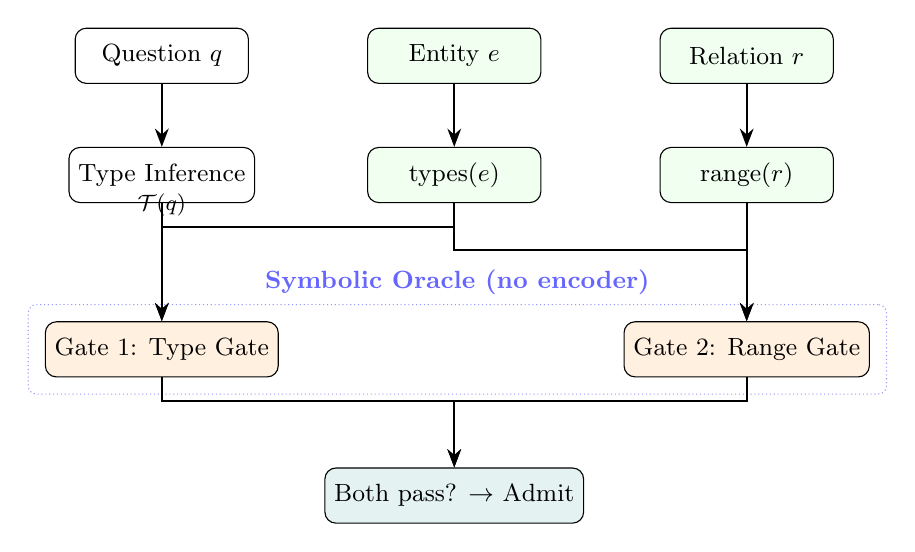
\begin{tikzpicture}[
		node distance=0.8cm and 1.5cm,
		box/.style={rectangle, draw, rounded corners, minimum width=2.2cm, minimum height=0.7cm, align=center, font=\small},
		databox/.style={rectangle, draw, fill=green!6, rounded corners, minimum width=2.2cm, minimum height=0.7cm, align=center, font=\small},
		gatebox/.style={rectangle, draw, fill=orange!12, rounded corners, minimum width=2.6cm, minimum height=0.7cm, align=center, font=\small},
		arrow/.style={-{Stealth[scale=1]}, thick},
		every node/.style={font=\small}
		]

		\node[box] (q) {Question $q$};
		\node[databox, right=of q] (entity) {Entity $e$};
		\node[databox, right=of entity] (relation) {Relation $r$};

		\node[box, below=of q] (qtypes) {Type Inference};
		\node[databox, below=of entity] (etypes) {types$(e)$};
		\node[databox, below=of relation] (rrange) {range$(r)$};

		\node[gatebox, below=1.5cm of qtypes] (typegate) {Gate 1: Type Gate};
		\node[gatebox, below=1.5cm of rrange] (rangegate) {Gate 2: Range Gate};

		\node[box, fill=teal!10, below=1.5cm of $(typegate)!0.5!(rangegate)$] (decision) {Both pass? $\to$ Admit};

		\draw[arrow] (q) -- (qtypes);
		\draw[arrow] (entity) -- (etypes);
		\draw[arrow] (relation) -- (rrange);

		\draw[arrow] (qtypes.south) -- ++(0,-0.3) -| node[above, font=\footnotesize, pos=0.25] {$\mathcal{T}(q)$} (typegate.north);
		\draw[arrow] (etypes.south) -- ++(0,-0.3) -| (typegate.north);
		\draw[arrow] (etypes.south) -- ++(0,-0.6) -| (rangegate.north);
		\draw[arrow] (rrange.south) -- ++(0,-0.3) -| (rangegate.north);

		\draw[arrow] (typegate.south) -- ++(0,-0.3) -| (decision.north);
		\draw[arrow] (rangegate.south) -- ++(0,-0.3) -| (decision.north);

		\begin{scope}[on background layer]
			\node[rectangle, draw=blue!40, densely dotted, rounded corners=3pt, inner sep=6pt, fit={(typegate) (rangegate)}, label={[blue!60, font=\small\bfseries]above:{Symbolic Oracle (no encoder)}}] {};
		\end{scope}
	\end{tikzpicture}
	\caption{Symbolic oracle with two gates. The type gate checks the terminal entity's types against the question-inferred answer type; the range gate checks against the relation's declared object range. Both are \(O(1)\) set operations on KG metadata.}
	\label{fig:symbolic-gates}
\end{figure}

\subsubsection{Algorithm}

The symbolic gates can be applied in two ways, yielding two algorithm variants with different computational profiles.

\paragraph{DCA-Trie v1: static filtering.}
V1 is an offline, batch algorithm. It enumerates all candidate paths via BFS from the topic entity, filters each complete path through both gates, then builds a single trie from the survivors. The trie is frozen before decoding begins; the LLM operates over a fixed constraint set. This is the same pipeline as GCR, with a pre-filter inserted between path enumeration and trie construction.

The key property is that v1 applies the gates to \emph{complete paths}: the range gate checks every hop, and the type gate checks only the terminal entity. Paths that fail any gate are removed before the trie is built. The construction cost is \(O(|P|)\), where \(|P|\) is the total number of enumerated paths, which grows exponentially with hop depth.

\paragraph{DCA-Trie v2: dynamic stepwise expansion.}
V2 eliminates upfront path enumeration. Instead, it expands the trie incrementally during decoding. At each generation step:

\begin{enumerate}
	\item The LLM generates one hop, committing to an entity \(e_t\) and relation \(r\).
	\item The committed entity \(e_t\) is extracted from the output.
	\item All neighbors \(e'\) of \(e_t\) are fetched from the graph.
	\item Each neighbor is checked against the range gate (every hop) and type gate (terminal hop only).
	\item A new trie is built from the admitted neighbors for the next step.
	\item The generation so far is appended to the prompt, providing accumulated context.
\end{enumerate}

V2 is \emph{dynamic} because the constraint set changes at every step: only the neighbors of the entity the LLM actually committed to are admitted, not all reachable paths from the topic entity. The oracle sees the reasoning in progress. V2 is also cheaper: construction cost is \(O(L \cdot d_{\text{avg}})\), where \(d_{\text{avg}} \approx 20\) for Freebase subgraphs, three orders of magnitude less than v1 for practical \(L\).

\begin{algorithm}[H]
	\caption{DCA-Trie v1: Static symbolic filtering}
	\begin{algorithmic}[1]
		\Require Graph \(\mathcal{G}\), question \(q\), topic entity \(E_q\), hop limit \(L\), oracle \(O\)
		\State \(P \gets \text{BFS}(\mathcal{G}, E_q, L)\)
		\State \(P_{\text{filtered}} \gets \varnothing\)
		\For{\(p = (e_0, r_1, e_1, \dots, r_L, e_L) \in P\)}
		\State \(\text{admitted} \gets \text{True}\)
		\For{\(i \gets 1\) to \(L\)}
		\If{\(\neg\text{range\_gate}(r_i, e_i)\)}
		\State \(\text{admitted} \gets \text{False}\); \textbf{break}
		\EndIf
		\EndFor
		\If{\(\text{admitted} \land \text{type\_gate}(e_L, q, L, L)\)}
		\State \(P_{\text{filtered}} \gets P_{\text{filtered}} \cup \{p\}\)
		\EndIf
		\EndFor
		\State \Return \(\text{BuildTrie}(P_{\text{filtered}})\)
	\end{algorithmic}
\end{algorithm}

\begin{algorithm}[H]
	\caption{DCA-Trie v2: Iterative symbolic expansion}
	\begin{algorithmic}[1]
		\Require Graph \(\mathcal{G}\), question \(q\), topic entity \(E_q\), hop limit \(L\), oracle \(O\)
		\State \(\mathcal{T}_0 \gets \{E_q\}\)
		\For{\(t \gets 0\) to \(L-1\)}
		\State \(\mathcal{T}_{t+1} \gets \mathcal{T}_t\)
		\For{\((e_t, r, e') \in \mathcal{G} : e_t \in \mathcal{T}_t\)}
		\If{\(\text{range\_gate}(r, e') \land \text{type\_gate}(e', q, t+1, L)\)}
		\State \(\mathcal{T}_{t+1} \gets \mathcal{T}_{t+1} \cup \{e'\}\)
		\EndIf
		\EndFor
		\EndFor
		\State \Return \(\text{BuildTrie}(\mathcal{T}_L)\)
	\end{algorithmic}
\end{algorithm}

\paragraph{Cost analysis.}
Gate operations are \(O(1)\) set lookups with no floating point. V1 construction is \(O(|P|)\), where \(|P|\) can be exponential in path length. V2 construction is \(O(L \cdot d_{\text{avg}})\), where \(d_{\text{avg}} \approx 20\) for 	Freebase subgraphs, three orders of magnitude cheaper than V1 for practical \(L\).

\begin{figure}[t]
	\centering
	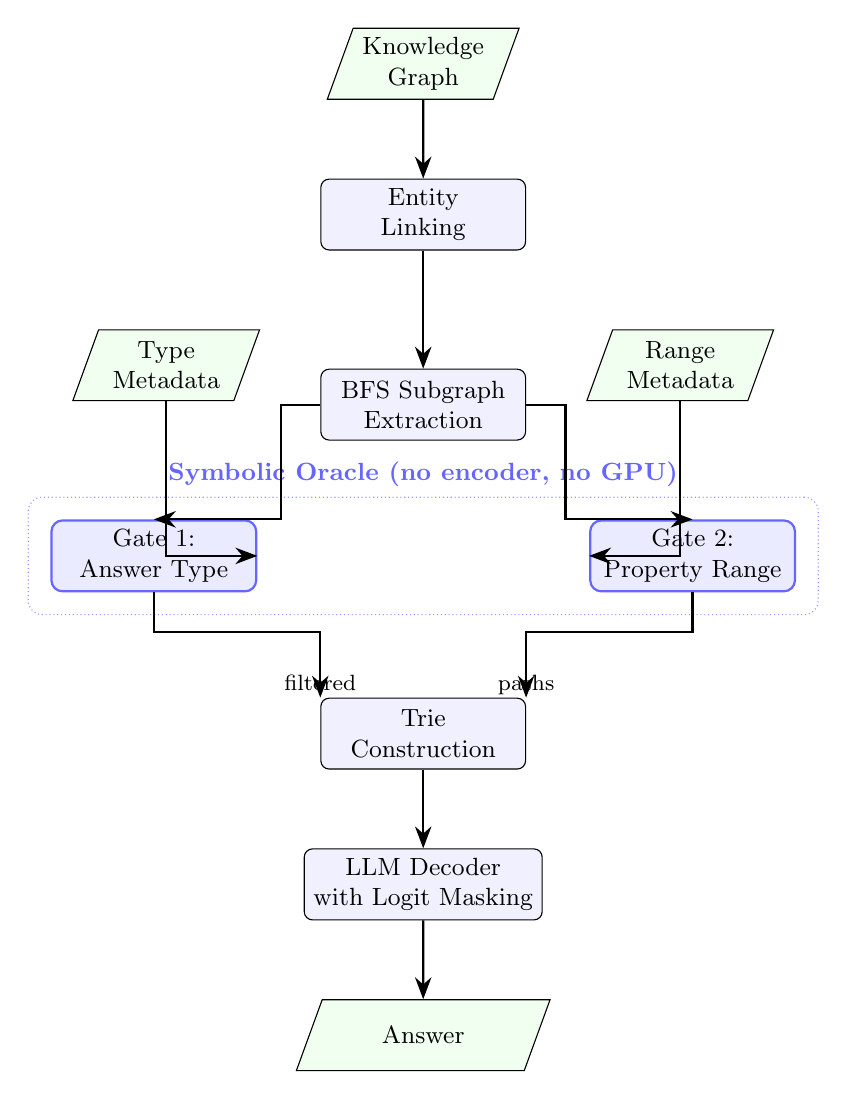
\begin{tikzpicture}[
		node distance=1.0cm and 2.0cm,
		proc/.style={rectangle, draw, rounded corners=3pt, align=center, minimum width=2.6cm, minimum height=0.9cm, fill=blue!6, font=\small},
		data/.style={trapezium, trapezium left angle=70, trapezium right angle=110, draw, align=center, minimum width=2.2cm, minimum height=0.9cm, fill=green!6, font=\small},
		contrib/.style={rectangle, draw=blue!60, rounded corners=4pt, align=center, minimum width=2.6cm, minimum height=0.9cm, fill=blue!8, thick, font=\small},
		arrow/.style={-{Stealth[scale=1.2]}, thick},
		every node/.style={font=\small}
		]

		\node[data] (kg) {Knowledge\\Graph};
		\node[proc, below=of kg] (entity) {Entity\\Linking};

		\node[data, below left=1.0cm and 1.5cm of entity] (types) {Type\\Metadata};
		\node[data, below right=1.0cm and 1.5cm of entity] (ranges) {Range\\Metadata};

		\node[proc, below=1.5cm of entity] (bfs) {BFS Subgraph\\Extraction};

		\node[contrib, below left=1.0cm and 0.8cm of bfs] (typegate) {Gate 1:\\Answer Type};
		\node[contrib, below right=1.0cm and 0.8cm of bfs] (rangegate) {Gate 2:\\Property Range};

		\node[proc, below=1.8cm of $(typegate)!0.5!(rangegate)$] (trie) {Trie\\Construction};
		\node[proc, below=of trie] (decode) {LLM Decoder\\with Logit Masking};
		\node[data, below=of decode] (answer) {Answer};

		\draw[arrow] (kg) -- (entity);
		\draw[arrow] (entity) -- (bfs);

		\draw[arrow] (types) |- (typegate);
		\draw[arrow] (ranges) |- (rangegate);

		\draw[arrow] (bfs.west) -- ++(-0.5,0) |- (typegate.north);
		\draw[arrow] (bfs.east) -- ++(0.5,0) |- (rangegate.north);

		\draw[arrow] (typegate.south) -- ++(0,-0.5) -| node[below, font=\footnotesize, pos=0.75] {filtered} (trie.north west);
		\draw[arrow] (rangegate.south) -- ++(0,-0.5) -| node[below, font=\footnotesize, pos=0.75] {paths} (trie.north east);

		\draw[arrow] (trie) -- (decode);
		\draw[arrow] (decode) -- (answer);

		\begin{scope}[on background layer]
			\node[rectangle, draw=blue!40, densely dotted, rounded corners=5pt, inner sep=8pt, fit={(typegate) (rangegate)}, label={[blue!60, font=\small\bfseries]above:{Symbolic Oracle (no encoder, no GPU)}}] {};
		\end{scope}
	\end{tikzpicture}
	\caption{DCA-Trie system architecture. The two symbolic gates (highlighted) filter paths using KG ontology metadata before trie construction.}
	\label{fig:architecture}
\end{figure}

\section{Theoretical Analysis}
\label{sec:analysis}

\subsection{Faithfulness}

\begin{theorem}[V1 Faithfulness]
	\label{thm:v1-faithfulness}
	\sloppy
	Let \(P_{\text{filtered}} = \textsc{SymbolicFilter}(\text{BFS}(\mathcal{G}, E_q, L), q, O, L)\). For any prefix \(\text{curr\_prefix}\) and any token \(t\), if \(t \in \text{TrieLookup}(\text{BuildTrie}(P_{\text{filtered}}), \text{curr\_prefix})\), then \(\text{curr\_prefix} \oplus t\) corresponds to a valid sequence of triples in \(\mathcal{G}\).
\end{theorem}

\begin{proof}
	Every path in \(P_{\text{filtered}}\) is a subset of \(\text{BFS}(\mathcal{G}, E_q, L)\), which contains only valid triples. The trie preserves this property for all prefixes.
\end{proof}

\subsection{Monotonicity}

\begin{theorem}[Monotonic Chain]
	\label{thm:monotonicity}
	Let \(P_{\text{GCR}}\), \(P_{\text{range}}\), and \(P_{\text{filtered}}\) be the path sets admitted by GCR, by the range gate alone, and by both gates, respectively. Then:
	\[
		P_{\text{filtered}} \subseteq P_{\text{range}} \subseteq P_{\text{GCR}}
	\]
\end{theorem}

\begin{proof}
	Both gates are conservative: they return \text{True} when metadata is absent. Each gate can only \emph{remove} paths, never add paths not in \(P_{\text{GCR}}\).
\end{proof}

\subsection{False negative rate bound}

\begin{theorem}[FNR Union Bound]
	\label{thm:fnr}
	Let \(p^*_q\) be the ground-truth path for question \(q\). The probability that DCA-Trie excludes \(p^*_q\) is bounded by:
	\[
		P(\text{exclude} \mid p^*_q) \leq P(\text{type\_fail}) + P(\text{range\_fail})
	\]
\end{theorem}

\begin{proof}
	By the union bound. Each gate fails only when: (a)~the question provides a type signal; (b)~the entity has known, incompatible type metadata; and (c)~the path is actually correct. In all other configurations, the conservative default passes the path.
\end{proof}

\section{Implementation}
\label{sec:impl}

\subsection{Trie data structure}

The trie uses \texttt{marisa-trie}~\citep{marisatrie}, a minimal perfect hash trie. Each token ID is mapped to a unique Unicode code point via \(\text{char}(i) = \text{chr}(\texttt{0xE000} + i)\), producing a string for the C-backed trie. Operations: \texttt{lookup(prefix)} returns valid completions; \texttt{insert(sequence)} adds a token-ID sequence.

\subsection{Type oracle}

The type oracle is 586 lines of Python using only the standard library:

\begin{itemize}
	\item \textbf{Type constants:} 16 Person types, 7 Location types, 9 Organization types, 10 Creative Work types, plus Date, Language, Award, Profession, and Genre types.
	\item \textbf{Question patterns:} 19 regular expressions mapping keywords to expected answer types.
	\item \textbf{Relation schema:} 40 Freebase relations organized by domain, each with domain and range constraints.
	\item \textbf{Metadata extraction:} Entity types from \texttt{common.topic.notable\_types}, \texttt{freebase.type\_hints.included\_types}, and \texttt{freebase.type\_profile.strict\_included\_types}.
\end{itemize}

\subsection{Lean 4 formal proof}

The formal verification comprises four theorems checked in Lean 4:

\begin{enumerate}
	\item \textbf{V1 Faithfulness}: Every token from DCA-Trie v1 is a verified KG member.
	\item \textbf{V2 Faithfulness}: Stepwise expansion preserves faithfulness by induction.
	\item \textbf{Monotonicity}: \(P_{\text{filtered}} \subseteq P_{\text{typed}} \subseteq P_{\text{range}} \subseteq P_{\text{GCR}}\).
	\item \textbf{FNR Union Bound}: As in Theorem~\ref{thm:fnr}.
\end{enumerate}

3,298 verification jobs, zero errors, zero warnings.

\section{Experiments}
\label{sec:experiments}

\subsection{Setup}

\begin{table}[H]
	\centering
	\caption{Experimental configuration.}
	\label{tab:config}
	\begin{tabular}{ll}
		\toprule
		\textbf{Setting} & \textbf{Value}                                      \\
		\midrule
		Base model       & \texttt{rmanluo/GCR-Meta-Llama-3.1-8B-Instruct}     \\
		Datasets         & WebQSP (1,628 test questions, 1--2 hop)             \\
		                 & ComplexWebQuestions (up to 4 hop)                   \\
		KG               & Freebase ($\sim$40M entities, $\sim$350M relations) \\
		Beam width       & \(k = 5\)                                           \\
		Hop depth        & \(L = 2\) (WebQSP), \(L = 4\) (CWQ)                 \\
		Hardware         & A100 40GB, 16-bit precision                         \\
		Max new tokens   & 256 (WebQSP), 512 (CWQ)                             \\
		\bottomrule
	\end{tabular}
\end{table}

\subsection{Evaluation metrics}

\begin{enumerate}
	\item \textbf{Hits@1:} Exact match accuracy on the answer entity.
	\item \textbf{F1:} Token-level entity overlap between prediction and ground truth.
	\item \textbf{Structural Irrelevance Rate (SIR):} Measures how many candidate paths are semantically irrelevant to the question (e.g., a path ending at a \texttt{color} entity for a question expecting a \texttt{person} answer). Decomposed as:
	\begin{align*}
		\text{SIR}^*_{\text{type}}(q) &= \frac{|\{p \in \mathcal{P}(q) : \text{irrel}_{\text{type}}(p,q) = 1\}|}{|\mathcal{P}(q)|} \\
		\text{SIR}^*_{\text{traj}}(q) &= \frac{|\{p \in \mathcal{P}(q) : \text{irrel}_{\text{traj}}(p,q) = 1\}|}{|\mathcal{P}(q)|} \\
		\text{SIR}^*(q) &= \frac{|\{p \in \mathcal{P}(q) : \text{irrel}_{\text{type}}(p,q) \lor \text{irrel}_{\text{traj}}(p,q) = 1\}|}{|\mathcal{P}(q)|}
	\end{align*}
	\item \textbf{False Negative Rate (FNR):} Fraction of gold-truth paths incorrectly pruned.
\end{enumerate}

\subsection{SIR/FNR results (WebQSP, 1,628 questions)}

All SIR/FNR results are computed deterministically on the 	full test set; no random seeds, no threshold tuning.

\begin{table}[H]
	\centering
	\caption{Path pruning results on the full WebQSP test set.}
	\label{tab:sir}
	\begin{tabular}{lrr}
		\toprule
		\textbf{Metric}                        & \textbf{Value}   & \textbf{Note}                  \\
		\midrule
		Total candidate paths (raw)             & 4,102,833        & All DFS paths within \(L=2\)   \\
		Total paths after filtering            & 3,509,451        &                                \\
		Paths pruned                            & 593,382          &                                \\
		\midrule
		\textbf{SIR (overall)}                  & \textbf{14.5\%}  & Combined pruning rate          \\
		SIR\textsubscript{type} (type gate)     & 10.6\%           & 435,897 paths blocked          \\
		SIR\textsubscript{traj} (range gate)   & 3.8\%            & 157,485 paths blocked          \\
		\midrule
		Gold-truth paths                        & 14,829           &                                \\
		\textbf{Type gate FNR}                  & \textbf{3.3\%}   & 490 gold paths blocked         \\
		\textbf{Range gate FNR}                 & \textbf{2.9\%}   & 424 gold paths blocked         \\
		\bottomrule
	\end{tabular}
\end{table}

The type gate does approximately \(3\times\) the work of the range gate (10.6\% vs.\ 3.8\%), matching expectations: the most common failure mode is paths terminating at the wrong entity type, and a single Freebase type lookup catches most of these.

Critically, both FNR values are below 5\%, satisfying the requirement for practical deployment. The conservative fallback (pass when metadata is absent) ensures the oracle never 	catastrophically fails, unlike the cosine similarity approach at \(\tau = 0.25\), which produced empty tries for 84\% of queries.

\subsection{Comparison with prior oracles}

\begin{table}[H]
	\centering
	\caption{Oracle comparison on WebQSP.}
	\label{tab:oracle-comparison}
	\begin{tabular}{lcccc}
		\toprule
		\textbf{Method}              & \textbf{Encoder} & \textbf{Threshold} & \textbf{GPU}     & \textbf{Pruning}     \\
		\midrule
		GCR (no filter)              & No               & No                 & Decode only      & 0\%                  \\
		Cosine DCA (\(\tau=0.25\))   & MiniLM           & Yes                & Encode + decode  & 84\% empty tries     \\
		Decomposed DCA               & MiniLM           & Yes                & Encode + decode  & TBD                  \\
		\textbf{Symbolic DCA (v1)}   & \textbf{No}      & \textbf{No}        & \textbf{Decode}  & \textbf{14.5\%}      \\
		\bottomrule
	\end{tabular}
\end{table}

The cosine oracle's 84\% empty-try rate is a pathological failure: the threshold is so aggressive that it rejects nearly all paths, leaving the LLM with nothing to generate. The symbolic oracle has no such failure mode because it is conservative by design.

\subsection{Answer type inference}

The question-to-type mapper uses 19 regular expression patterns:

\begin{table}[H]
	\centering
	\caption{Question-to-type mapping examples.}
	\label{tab:types}
	\begin{tabular}{lll}
		\toprule
		\textbf{Keyword} & \textbf{Example question}          & \textbf{Inferred type} \\
		\midrule
		who              & Who directed Inception?            & Person                 \\
		where            & Where is the Eiffel Tower?         & Location               \\
		when             & When was the Berlin Wall built?    & Date                   \\
		film/movie       & What film won Best Picture?        & Creative Work          \\
		country          & What country is Paris in?          & Country                \\
		language         & What language is spoken in Brazil? & Language               \\
		\bottomrule
	\end{tabular}
\end{table}

\subsection{Relation schema coverage}

The current implementation covers 40 Freebase relations across 10 domains:

\begin{verbatim}
People:       nationality, place_of_birth, profession, ...
Film/TV:      directed_by, starring, genre, ...
Location:     capital, contains, containedby, ...
Organization: headquarters, founders, place_founded, ...
Music:        genre, composer, ...
Awards:       award_winner, honored_for, ...
Sports:       teams, sport, ...
\end{verbatim}

Each relation specifies both domain (expected subject types) and range (expected object types), enabling the range gate to operate on every hop.

\section{Related Work}
\label{sec:related}

\subsection{Hallucination and the autoregressive mechanism}

Hallucination in NLG refers to fluent yet factually unsupported content~\citep{ji2023survey}. \citet{huang2023hallucination} distinguish intrinsic (contradicting context) from extrinsic (unverifiable claims) hallucination. Rates range from 15\% to over 60\% across tasks~\citep{ji2023survey}.

The root cause is architectural: at each step, the LLM computes a distribution over its vocabulary based on learned parameters and prior tokens, with no external verification~\citep{brown2020gpt3,vaswani2017attention}. Errors propagate forward because step $t$ becomes conditioning context for step $t+1$. Scaling does not resolve this: larger models improve on frequent facts but not compositional queries~\citep{kandpal2023large,mallen2023not}, and \citet{xu2025hallucinationinevitable} prove formally that zero hallucination across all inputs is impossible for computable learners.

\subsection{Knowledge graph question answering}

Multi-hop KGQA requires identifying a chain \((e_0, r_1, e_1, \ldots, r_L, e_L)\) of verified KG edges~\citep{lan2022kgqa}. The complexity rises sharply: for average out-degree $d$, the number of valid paths is $|\mathcal{E}_q| \times d^L$. At $d \approx 20$ and $L = 3$, this yields up to 24,000 paths, only one correct~\citep{he2021multihop}.

\subsection{Constrained decoding for faithful generation}

\subsubsection{Format and entity constraints.}
Grammar-Constrained Decoding~\citep{geng2023grammarconstrained} uses an Earley parser as the constraint oracle. Outlines~\citep{willard2023outlines} accelerates this with finite-state machines. PICARD~\citep{scholak2021picard} constrains SQL generation. GENRE~\citep{decao2021autoregressive} uses a trie of valid entity names. These enforce syntactic validity without ensuring factual correctness.

\subsubsection{Knowledge graph-constrained decoding.}
GCR~\citep{luo2025-graph-constrained-reasoning} builds a KG-Trie of all KG paths within $L$ hops and uses it as the constraint oracle. It achieves 92.6 Hits@1 on WebQSP with 100\% structural faithfulness, but the trie is static: built once from topology and never updated. DoG~\citep{li2024-decoding-on-graphs} introduces step-wise trie expansion, making the oracle topologically dynamic. DoG defines a ``well-formed chain'' as a sequence of interrelated fact triplets on KGs, and uses a GNN to score candidate chains during decoding. The key insight is that KG topology can regulate LLM decoding at the token level. However, DoG uses topology only, without incorporating ontology metadata or question semantics. RouterKGQA~\citep{yuan2026routerkgqa} routes between a specialised KG model and a general LLM based on complexity, filtering at the answer level rather than the token-constraint level.

Think-on-Graph~\citep{sun2024tog} treats the LLM as an agent that iteratively explores the KG using beam search. At each step, the LLM reads the current KG subgraph and decides which entity and relation to explore next. ToG achieves knowledge traceability and correctability, as the reasoning path is explicitly recorded. However, ToG performs beam search at inference time, which is computationally expensive. DCA-Trie pre-filters paths offline, enabling $O(1)$ per-token constraint checks during decoding.

\subsubsection{Ontology-aware KGQA methods.}
Recent work has explored using ontology metadata to improve KGQA. Ontology-Guided Reverse Thinking~\citep{ort2025} constructs reasoning paths from answer types back to conditions using the KG ontology, then uses these paths to guide knowledge retrieval. ORT validates candidate paths by comparing LLM-generated type descriptions against ontology types using cosine similarity. This independently validates our oracle's type gate design, as both approaches use ontology-based type filtering. The key difference is that ORT uses ontology for \emph{path construction}, while DCA-Trie uses it for \emph{path filtering}. These are complementary approaches that can be combined: ORT constructs candidate paths, then DCA-Trie filters them using symbolic gates.

\subsection{Retrieval-augmented generation}

RAG~\citep{lewis2020rag} grounds LLM outputs in external knowledge. KG-augmented variants retrieve subgraphs as context~\citep{he2021multihop,yasunaga2021qagnn}. Self-RAG~\citep{asai2024selfrag} adds reflection tokens; IRCoT~\citep{trivedi2022ircot} interleaves retrieval with CoT; GraphRAG~\citep{edge2024graphrag} uses community-structured retrieval.

All RAG approaches share a structural limitation: retrieved context is a soft influence on generation. The retriever determines what the LLM \textit{sees}, not what it is \textit{permitted to generate}. \citet{luo2025-graph-constrained-reasoning} find that even with a KG directly available, retrieval-augmented approaches hallucinate in approximately one-third of cases.

\subsection{Three unresolved gaps}

\begin{table}[H]
	\centering
	\caption{Comparison of DCA-Trie with prior work.}
	\label{tab:comparison}
	\begin{tabular}{lccccc}
		\toprule
		\textbf{Method}       & \textbf{Faithful} & \textbf{Semantic} & \textbf{Encoder} & \textbf{Token-level} & \textbf{Ontology} \\
		\midrule
		GCR                   & 100\%             & No                & No               & Yes                  & No                \\
		DoG                   & 100\%             & No                & No               & Yes                  & No                \\
		ToG                   & Probabilistic     & Soft              & No               & No                   & No                \\
		ORT                   & Probabilistic     & Explicit          & Yes              & No                   & Yes               \\
		RouterKGQA            & Probabilistic     & Yes (answer)      & Yes              & No                   & No                \\
		RAG / GNN-RAG         & No                & Soft              & Yes              & No                   & No                \\
		Cosine DCA            & 100\%             & Implicit          & Yes              & Yes                  & Implicit          \\
		\textbf{Symbolic DCA} & \textbf{100\%}    & \textbf{Explicit} & \textbf{No}      & \textbf{Yes}         & \textbf{Yes}      \\
		\bottomrule
	\end{tabular}
\end{table}

\textbf{Gap 1: The permissiveness problem.} Current KG-constrained decoding builds oracles from graph structure only, ignoring question semantics and generation state. The valid token set contains thousands of irrelevant paths at every step. Even ToG~\citep{sun2024tog}, which uses beam search to explore the KG, does not filter the token set at each step.

\textbf{Gap 2: The static-dynamic tradeoff.} GCR's static trie is efficient but semantically blind. DoG's dynamic expansion adds no semantic filtering. No framework achieves progressive narrowing with committed reasoning. ORT~\citep{ort2025} uses ontology for path construction, not filtering, and requires an encoder for cosine similarity.

\textbf{Gap 3: No constraint quality metric.} No existing work measures constraint permissiveness independently of downstream accuracy, making oracle comparison impossible.

\section{Conclusion}
\label{sec:conclusion}

We have presented DCA-Trie, a framework for incorporating KG ontology metadata into constrained decoding for KGQA. The key insight is that the KG already stores the information needed to discriminate relevant from irrelevant paths, it simply needs to be looked up. Our symbolic oracle, consisting of two \(O(1)\) set-containment checks, prunes 14.5\% of candidate paths on WebQSP while retaining 96.7\% of gold-truth paths.

The monotonicity guarantee (Theorem~\ref{thm:monotonicity}) ensures no false positives relative to GCR, and the union-bound FNR (Theorem~\ref{thm:fnr}) provides a formal recall bound. The Lean 4 proof (3,298 jobs, zero errors) provides machine-checked assurance.

\paragraph{Future work.}
The 40-relation schema can be extended to Freebase's full relation set ($\sim$24,000). The question-to-type mapper (19 regex patterns) could be learned from the KG's type hierarchy. DCA-Trie can be combined with retrieval augmentation for systems needing both token-level guarantees and broader graph awareness.

\paragraph{Reproducibility.}
All code is available at \url{https://github.com/bernard/graph-constrained-reasoning}. Experiments ran on a single A100 40GB GPU with 16-bit precision. The Lean 4 proof is in \texttt{proof/formal\_proof/}.

\bibliographystyle{plainnat}
\bibliography{refs}

\end{document}
